\documentclass[10pt,a4paper]{article}
\usepackage[utf8]{inputenc}
\usepackage{amsmath}
\usepackage{amsfonts}
\usepackage{amssymb}
\usepackage{graphicx}
\usepackage{subfigure}
\usepackage{amsmath}
\usepackage{mathrsfs}
\DeclareRobustCommand{\orderof}{\ensuremath{\mathcal{O}}}
\bibliographystyle{prsty}
\usepackage[top=1in, bottom=1in, left=1in, right=1in]{geometry}
\begin{document}
\section{What is PiLab?}
PiLab\footnote{PiLab is a part of a library called the ``PiLib". PiLab is to  provide users an integrated input and output interface to solve particular tasks using the subroutines collected in PiLib. Therefore, ``PiLib" may appear frequently in output files but it is not a typo.} is a Scilab\footnote{Scilab is a free and open-source matlab-like scientific computing language. Many resources can be found in http://www.scilab.org. } based code that calculates condensed matter problems for periodic (so called $\pi$-Lab) lattice systems using tight-binding approaches.\\

\textbf{What Can PiLab Do?} \\

 The current version PiLab-0.7.0 provides the following functions:\\

- Core Layer:
\begin{itemize}
\item Periodic lattice structure construction
\item Generaion of hopping integrals using Slaster-Koster methods
\item Basis transformation (relativistic/non-relativistic, cubic/spherical)  
\item Spin-orbit interactions
\item Self-Consistent TB+U and Fermi level calculations.
\end{itemize}

- Application Layer:
\begin{itemize}
\item Band structure 
\item Density of state
\item Floquet Hamiltonian
\item Chern number
\item Z2 invariant  (Testing)
\item Mapping of Multipolar Exchange Interaction (Testing)
\item Defect state (Testing)
\item Quantum Transport using surface Green's function method (Testing)
\end{itemize} 

- Extension Layer:
\begin{itemize}
\item Floquet band structure
\item Floquet Chern number
\item Floquet Z2 invariant (Testing)
\end{itemize}

More functions will be added in the near future. \\

\textbf{Features of PiLab}
\begin{itemize}
\item Easy Graphing: Thank to the powerful graphic ability of Scilab, PiLab can let you view your calculation results immediately
\item Easy Extracting: PiLab is designed to output all calculation results in an unified format. It also provides several functions to help you load and pass these data to other program. So you can easily extract the calculated data from PiLab and use your own codes for further data processing. 
\item Easy Extending: PiLab uses an open framework. It also provides tools for you to easily add your own code to PiLab. So you can extend PiLab base on the current functions to deal with tasks that are not supported without understanding the other part of PiLab.
\end{itemize}

\section{Installation}
In the following, we will use a few notations to help the user understand how to use PiLab. 'ABC' means a string \textbf{ABC} in scilab console and we will leave ``ABC'' as the usually meaning of a quotation mark. " $\rightarrow ABC$ " means to input ABC as a command in the console of Scilab. 

To install PiLab, you must install Scilab first. The latest version of Scilab can be found here: http://www.scilab.org. Once Scilab is installed, follow the instruction to install PiLib.
\begin{itemize}
\item Download PiLib source code from http://sites.google.com/site/pilabproject/
\item Unzip the file and put it to somewhere you like, say, /User/PiLib/
\item Open the file scilab.start. In windows, it should be in C:/Program Files/scilab-5.5.0/etc, in Linux, it should be in /scilab-5.4.0/share/scilab/etc. 
\item Find this comment in the file. \\

\textit{// Protect variable previously defined  } \\
 
 Add the following command just below this comment and \textbf{before the keyword predef("all")}\footnote{If you are a developer of PiLib, you should not include \textit{exec(PiLib);} because the \textit{predef("all")} command will prohibit you to reload PiLib promptly. Instead, you should run $\rightarrow$ exec(PiLib) every time you want to use PiLib} \\
 
\textit{PiLib\_path='/User/PiLib/';}  

\textit{PiLib=PiLib\_path+'PiLib\_loader.sce';} 

\textit{exec(PiLib);}

\item Open Scilab, if there is no any error message, your installation should be correct. To test it, let's try to execute the cubic harmonic spin-1 tensor operator generator in PiLib:

$\rightarrow$ \textit{PIL\_TO\_gen(1,'c')}

if it gives you nine 3x3 matrices, it works perfectly.  

\end{itemize}

\section{Framework of PiLab}

\subsection{Layer Sturcture}
All tasks in PiLab are called by a file named by the format \textbf{project\_task.plb}. 
For example, if one has a project called ``Graphene" and wants to generate its lattice structure, it should be named as ``Graphene\_lat.plb" where ``lat" is the keyword for lattice construction in PiLab. Other keywords for tasks like ``hop" (hopping interal), ``scc" (self-consistency), etc. 

PiLab uses a layer structure which means all tasks are classified into a layer. Tasks in lower layer require the completion of higher layer. There are three layers, ``core layer", ``application layer" and ``extension layer". Core layer is the basic layer. It defines the crystal lattice and generate the corresponding electronic structures. All the tasks in other layer will need the completion of all the tasks in this layer. In summary, it does three things: 1). lattice structure construction (lat), 2). generation of hopping integrals (hop) and 3). self-consistent calculation (scc). The order of the tasks in core layer cannot be changed, so you cannot do task \textbf{hop} before task \textbf{lat}. 

As for the application layer, it contains several tasks that can calculate the physical properties form the results of core layer (electronic structure) directly. All the tasks in this layer are independent and will not influence each other. The only requirement is one has to complete all core layer calculations. Tasks in this layer are band structure calculation (ban), density of state (dsn), Floquet Hamiltonian (flq), Chern number (chn), etc. 
\begin{figure}[tbp]
\centering
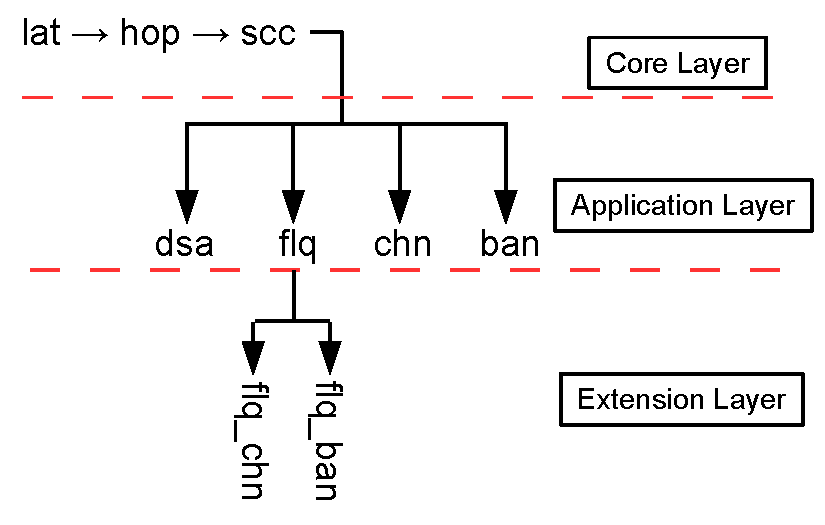
\includegraphics[width=0.8\columnwidth]{flow_chart.pdf}
\caption{Task flow chart of PiLab-0.7.0}
\end{figure}

Although the application layer can give us many physical properties, some properties cannot be obtained directly from the electronic structures. For example, Floquet problem, modification the electronic structure by shinning a light, requires one to calculate the Floquet Hamiltonian first. Once the Floquet Hamiltonian is obtained, the Floquet band and Floquet Chern number can be calculated. So those functions cannot be included in the application layer. Therefore, I introduce the extension layer. The extension layer contains the extended calculations of a particular task in the application layer. To avoid confusion, all the task name in this layer will have the form ``app\_ext" where ``app" means the corresponding task in the application layer and "ext" means the task in extension layer. For example, task name "flq\_ban" means to calculate the Floquet band structure form the "flq" results. Also, "flq\_chn" means to calculate the Floquet Chern number from the "flq" results. A flow chart of PiLab tasks of the version 0.7.0 is shown in Fig.1 and the meaning of each task keyword are listed below:\\

\textbf{Core level } \\

lat: lattice structure generation\\

hop: hopping integrals generation\\

scc: self-consistent calculation\\

\textbf{Application level } \\

ban: band structure calculation\\

dsa: density of state spectrum\\

flq: Floquet Hamiltonian generation \\

chn: Chern number calculation \\

\textbf{Extension level } \\

flq\_ban: Floquet band structure calculation \\

flq\_chn: Floquet Chern number calculation \\

Since this document just introduce the framework of PiLab, we will not change this flow chart or the list of task keywords if new function are released. Instead, we will just update \textbf{PiLab Dictionary}, another document that describes the details of each task. 

\subsection{Input and Output}
The basic logic of PiLab is that one prepares an input file of a task. Then run PiLab to perform corresponding calculations. When it is done, all calculation results will be appended to the input file. Hence the task file \textbf{project\_task.plb} will store not only the input but also the output information. If we perform next task, the task file will automatically read all necessary \textbf{.plb} files (at the same time, generates many temporary files with extension \textbf{.sod}) to continue new calculation. Note that, when performing a task, PiLab will generate many files with extension \textbf{.sod}. It stores the binary data of each \textbf{.plb} file. They are just temporary files during the calculations and you can delete it if you don't want them. It won't affect any calculation.   

To demonstrate the input and output structure of PiLab, we will begin with a baby calculation, a lattice structure calculation of two-diemnsional Graphene. To this end, first you have to prepare an input file \textbf{Graphene\_lat.plb}. PiLab has a useful function \textbf{PiLab\_create} to help users generate template files for all tasks. For some tasks, this function will also set appropriate default values for some parameters. 

To generate \textbf{Graphene\_lat.plb}, type the command in Scilab console (you should create a folder to collect all your project file and \emph{change the Scilab working folder to there}):\\

$\rightarrow$ \textit{PiLab\_ create('Graphene','lat')}\\ \\
Then PiLab will generate a file Graphene\_ lat.plb in the working folder. This file can be opened and edited by any text editors (It is highly recommend to use Notepad++ or Pspad if you are using Windows platform because they can help you manage projects easily). In the file, there should be: \\

lat.Const=[ ]\quad \quad \quad \quad \quad	// lattice constant, 1x1 real 

lat.Primitive=[ ] \quad \quad \quad // Primitive vectors, (3x3/2x2/1x1)

lat.Sublatt=[ ] \quad \quad \quad \quad // sublattice position, (nx3/nx2/nx1/)

lat.Order=[ ]\quad \quad \quad \quad \quad // Nearest Neighbor Order, 1x1 integer \\

A typical input file will look like this. There are few input syntax lat.Xxxx. The square brackets are where to put the input values. The words after ``//" are comments which will not be read by PiLab. One may also notice that all sub-syntax are capitalized in their initial, e.g lat."C"onst, lat."P"rimitive, etc. This is a convention in PiLib. If you wants to generate a input file by yourself instead of using the built-in PiLab\_create function, be sure to make it correct. 

I'm not going to explain the meaning of each parameter at this stage. For the meaning and the details, please check PiLab Dictionary. Now, input the values for each parameters (Note, comma "," and semicolon ";" are different! If you are a Matlab user, you should know their difference): \\

lat.Const=[1]  \qquad \qquad \qquad \qquad \qquad \qquad \qquad  // lattice constant, 1x1 real 

lat.Primitive=[-3/2,sqrt(3)/2;3/2,sqrt(3)/2] \quad // Primitive vectors, (3x3/2x2/1x1)

lat.Sublatt=[0,0;1,0] \qquad \qquad \qquad \qquad \qquad \quad //sublattice position, (nx3/nx2/nx1/)

lat.Order=[2]\qquad \qquad \qquad \qquad \qquad \qquad \qquad // Nearest Neighbor Order, 1x1 integer \\

Save it, then type the command in Scilab console (make sure you are in correct working folder):\\

$\rightarrow$ PiLab('Graphene','lat')\\

When the calculation is done, check \textbf{Graphene\_lat.plb} again, you will find the file has been modified. The calculation results has been appended to the file as shown in Fig.2.   
\begin{figure}[tbp]
\centering
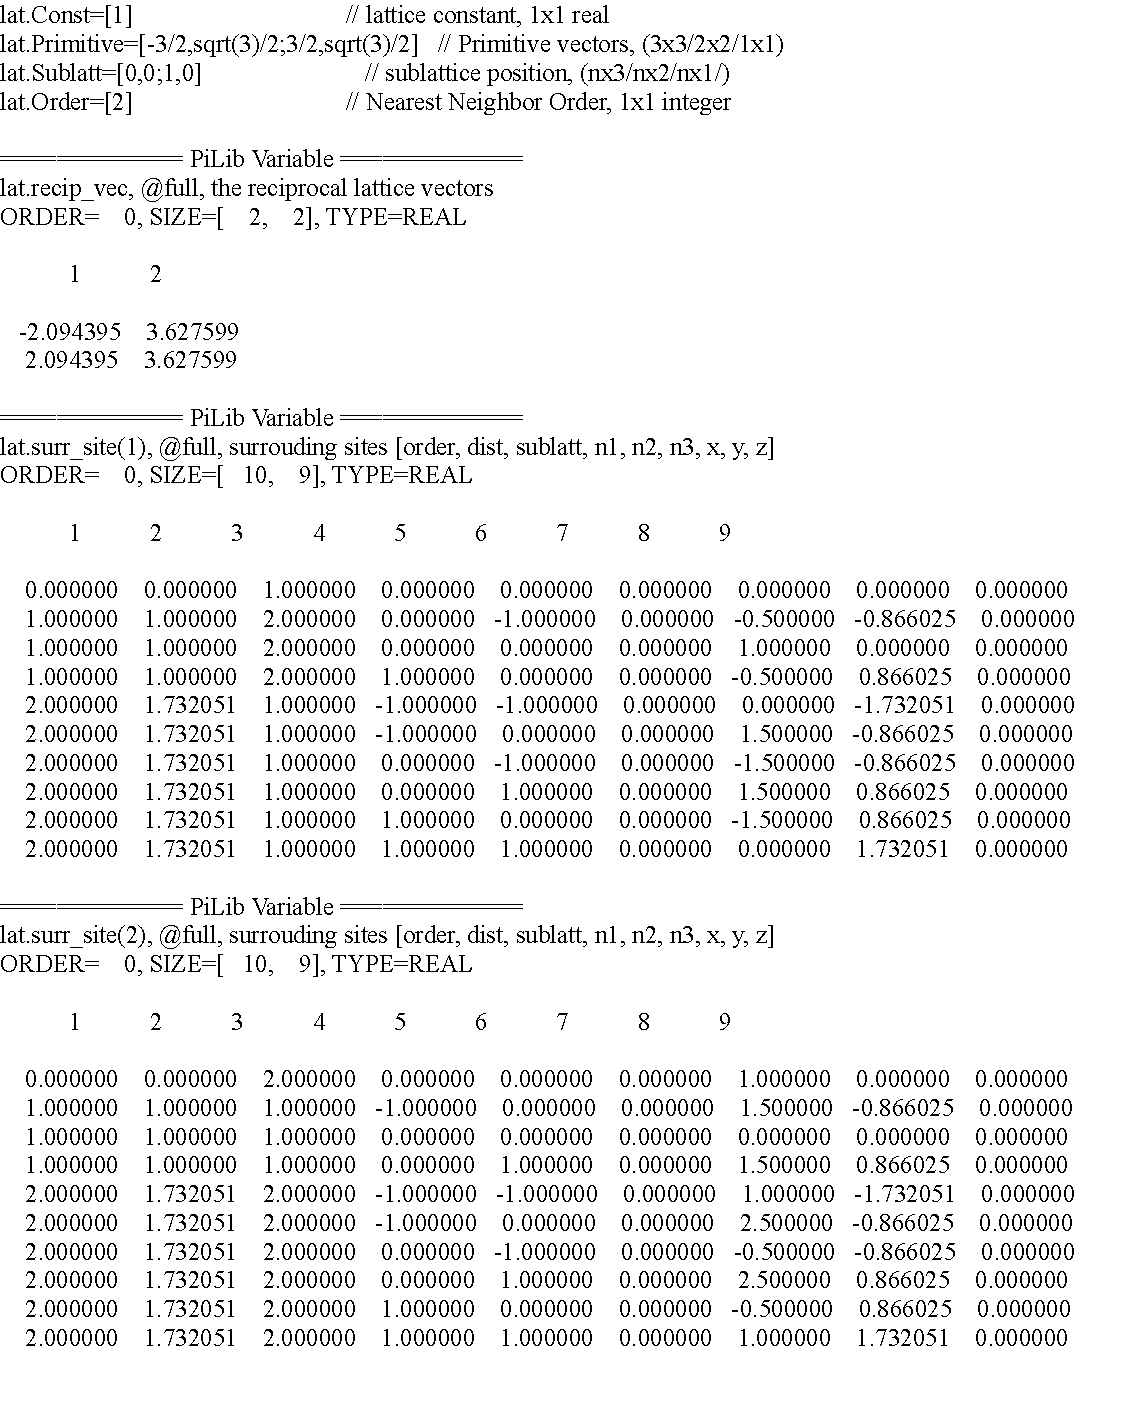
\includegraphics[width=1.0\columnwidth]{Graphene_lat.pdf}
\caption{Graphene\_lat.plb}
\end{figure}     
In the appended part, one can immediately find all the output variables start with a statement:\\ \\
============= PiLib Variable =============\\ \\
This is a conventional statement of the PiLib. All the variable in PiLab is a matrix and PiLib will output them with this header. Just below it, there are two explanation line. Taking the first variable as an example:\\ \\
lat.recip\_vec, @full, the reciprocal lattice vectors \\
ORDER=    0, SIZE=[    2,    2], TYPE=REAL    \\

The first line contains three information. The first is the variable name: \textbf{lat.recip\_vec}. It is the variable name that used in the code. "@full" means the output data is a full matrix rather than a sparse matrix (there are three output format, @full, @a-sp, @t-sp. Their difference will be introduced in next section). \textbf{the reciprocal lattice vectors} is a short comment of this variable, so users can understand the meaning of this output data. The second line contains the information of its numerical properties. Because all PiLib variables are output using scientific notation. Therefore, all values in PiLib variables range between $\pm 0.000000 \sim \pm 1.000000 \times 10^{n}$. Here \textbf{ORDER=    0} means all the output matrix elements have to multiply $10^{0}$. \textbf{SIZE=[    2,    2]} means the output matrix has a size of 2x2. \textbf{TYPE=REAL} means the output matrix are real values. There are other output types, e.g COMPLEX, SPARSE. For details, see next section. After the explanation line, comes the column number line. This is nothing but the column number of your output matrix. The matrix:\\ \\
-2.094395 \quad   3.627599 \\
\quad 2.094395 \quad   3.627599 \\ \\
is the output data. Combine all information, the first variable can be understood as: 1) the variable name is \textbf{lat.recip\_vec} 2). it is a full matrix rather than a sparse matrix 3). this variable describes the reciprocal lattice vectors 4). this matrix has to multiple $10^{0}$ 5). This is a 2x2 matrix 6). This is a real value matrix. 7). The matrix elements are [-2.094395, 3.627599 ; 2.094395, 3.627599 ] which means the two reciprocal lattice vectors are [-2.094395, 3.627599] and [2.094395, 3.627599] respectively. 

Therefore, to perform a task in PiLab, all you have to do is to understand the meaning of each input parameters and give them appropriate values. Then understand the meaning of each output variables. The details of each task should consult \textbf{PiLab dictionary} which can be found on the official website.  

A very important concept in PiLab is that \textbf{one can always manually change the output data and perform all later calculations based on the manually changed results}. It allows users to deal with special problems where their hopping integrals or density matrices cannot be obtained by simple Slaster-Koster scheme. An interesting example is Haldane model where the second nearest hopping integrals are modified by a magnetic field with net flux equal to zero. This example can be found in the \textbf{PiLab example depot} on the official website. 

\section{Output Format}
In the last section, we have mentioned there are several format of the output data. In fact, there are three types to output a matrix: @full, @t-sp, @a-sp, and four numerical types: STRING, REAL, COMPLEX, SPARSE. The reason that I introduce these types is to make the output data more concise and readable. In Fig.3, typical output format of each combination has been shown. Consider we have a NxM matrix. If this matrix has no special property, the easiest way is to output the whole matrix as found in the variable \textbf{lat.recip\_vec} of Fig.3. However, it is possible that the matrix are zero everywhere except some matrix elements. If so, a better way to show the matrix is to output the locations and the values of non-zero matrix elements only. This idea is called sparse matrix. It is what @a-sp does (all + sparse, so called @a-sp). Futhermore, if the matrix is sparse and hermitian, we can even show the non-zero matrix elements of the upper triangle part only. It is what @t-sp does (triangle + sparse, so called @t-sp).

As for the numerical type: STRING, REAL, COMPLEX, SPARSE. there are nothing special and one should easily understand their meaning. Just remember that for @a-sp or @t-sp format, PiLib will show the indies and the values of the non-zero matrix elements rather than the whole matrix. In Fig.3, \textbf{hop.hop\_mat(1)(:,:,3)} is a @a-sp matrix. For a sparse matrix, \textbf{SIZE=[ 2, 3]} means the matrix in sparse format is 2x3. It doesn't mean the full matrix is 2x3. In first row of the output data: 2 2 0.000000 0.000000 means the full matrix is 2x2 and 0.000000 0.000000 has no meaning (just for alignment). The below part shows the indies and values of the non-zero matrix elements. Therefore, the output data demonstrates the variable \textbf{hop.hop\_mat(1)(:,:,3)} is a 2x2 matrix and the only non-zero matrix element is (1,2) and its value is 1.000000+0.000000i (by default, all sparse matrices are shown as complex values). Similar case can be found in \textbf{scc.DM\_out}. However, this is a @t-sp variable, so the output data are just its upper triangle.

Examples of COMPLEX and STRING can be found in \textbf{ban.k\_vec(:,:,1)} and \textbf{hop.state\_info\_text}. For COMPLEX, each matrix element is represented by two real values. The first one is the real part and the second one is the imaginary part. As for STRING, because a blank '   ' can also be a part of a string, so PiLib uses the notation "\#" to separate each string.  
  
\begin{figure}[tbp]
\centering
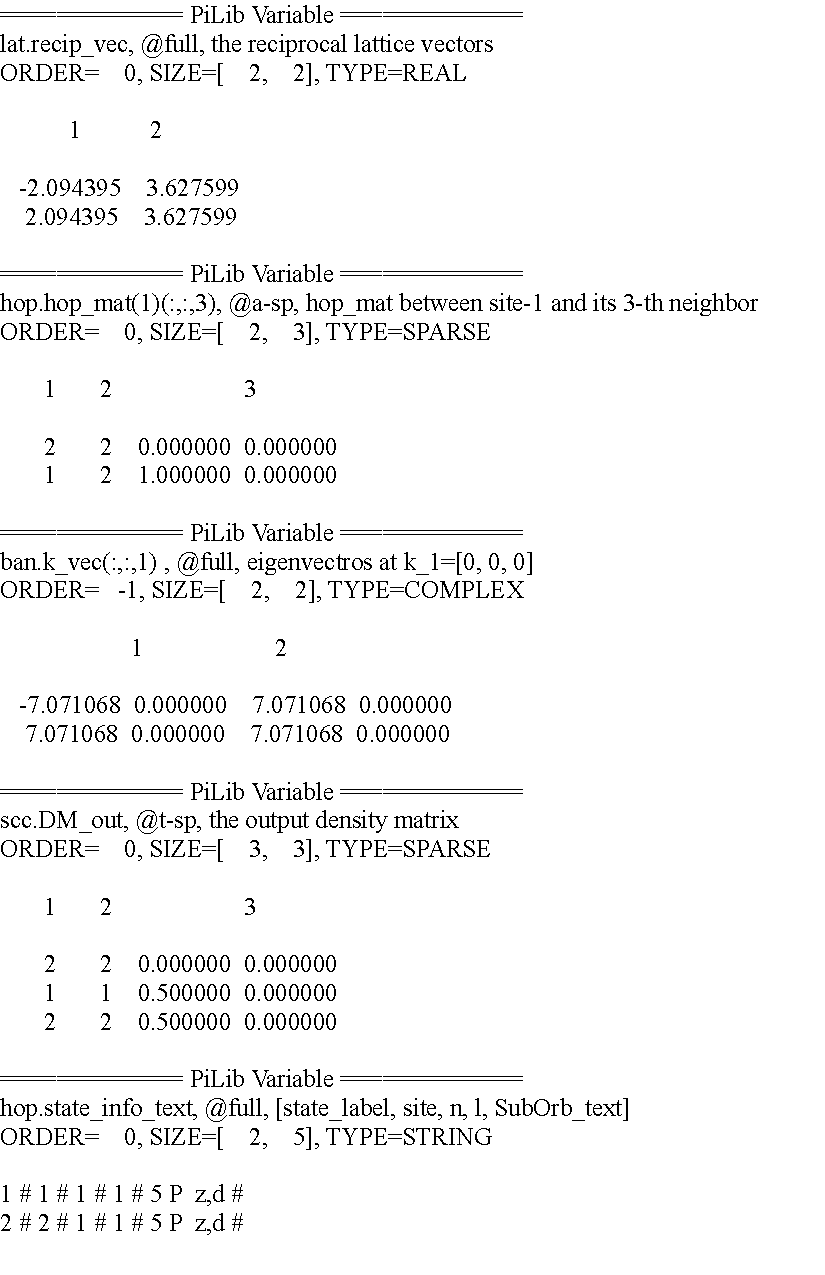
\includegraphics[width=0.8\columnwidth]{output_format.pdf}
\caption{output format}
\end{figure}

\section{Exercise}
In this section, I will lead you to have a quick exercise. Let's try to calculate the band structure, the density of state and the Chern number, etc, of a graphene. All the input files are prepared and can be downloaded from the official website (see Graphene folder in PiLab Example Depot section). You may find there are several files named \textbf{Graphene\_xxx.plb}. The meaning of the input parameters and the output variables can be found in the \textbf{PiLab dictionary}. Here I will just lead the users to run this project. One should also reference PiLab dictionary when a task is performed.    

First we will need to complete all core layer tasks. As mentioned in the previous sections, the tasks in core layer have to follow the order \textbf{lat $\rightarrow$ hop $\rightarrow$ scc}. Therefore, follow the steps:
\begin{itemize}
\item change the working folder of Scilab to the folder where you put all the \textbf{.plb} files
\item $\rightarrow$ PiLab('Graphene','lat')
\item $\rightarrow$ PiLab('Graphene','hop')
\item $\rightarrow$ PiLab('Graphene','scc')
\end{itemize}
While perform each step, one should also check the changes of each \textbf{.plb} files and reference the \textbf{PiLab dictionary} for the meaning of each output variable. Once the above steps are done. We can now perform \textbf{.ban}, \textbf{.dsa}, \textbf{.chn} and \textbf{flq}. Since each task in application level are independent, one can perform these tasks with arbitrary order.
\begin{itemize}
\item $\rightarrow$ PiLab('Graphene','ban')
\item $\rightarrow$ PiLab('Graphene','dsa')
\item $\rightarrow$ PiLab('Graphene','chn')
\item $\rightarrow$ PiLab('Graphene','flq')
\end{itemize}
While perform \textbf{ban} and \textbf{dsa}, PiLab will also draw the band structure and density of state. You can check them with the results obtained form  the analytical solutions of the 2x2 graphene Hamiltonian which has been formulated by many textbooks. One can also perform Floquet band and Floquet Chern number calculations . 
\begin{itemize}
\item $\rightarrow$ PiLab('Graphene','flq\_ban')
\item $\rightarrow$ PiLab('Graphene','flq\_chn')
\end{itemize}
Note that, \textbf{flq\_ban} and \textbf{flq\_chn} are tasks in the extension layer. Their father task is \textbf{flq}. If it is not performed first, \textbf{flq\_ban} and \textbf{flq\_chn} will not be able to run.   

\section{Loading Data}
It is likely that you just want to use part of the functions in PiLab and use your own codes for further data processing. If so, use the function: \textbf{PiLab\_loader('project','task')}. For example, if you want to load the data in \textbf{graphene\_hop.plb} file, just use\\ \\
$\rightarrow$ PiLab\_load('graphene','hop') \\ \\
Then all the data including inputs and outputs will automatically be stored in a file named \textbf{graphene\_hop.sod}. This is a Scilab binary format file. To load it into the Scilab workspace, use:\\ \\
$\rightarrow$ load('graphehe\_hop.sod') \\ \\
Now it becomes a normal variable in Scilab workspace named \textbf{hop}, so can use any Scilab allowed methods to handle the data.  
\section{Conclusion}
All the basic concepts of PiLab have been introduced in this article. The main idea of using PiLab is 1). prepare the input file using \textbf{PiLab\_create} function 2). understand the meaning of output data 3). perform each task based on the flow chart as shown in Fig.1. PiLab will continue to develop new functions and make it more flexible to deal with various condensed matter problems. However, unless needed, we will not update this document frequently because the framework of PiLab will not change. Instead, we will update the \textbf{PiLab dictionary} and \textbf{PiLab example depot}. These resources can be found in the official website of PiLab.

%\section{Acknowledge}
%This project was accomplished while I was a PhD student in Prof.Savrasov's group in the Physics Departemnt of UC Davis. I would like to thank for anyone who helped me during my academic life particularly my family and my advisor. 
%
%\section{Copyright}
%This code can be distribution  
\end{document}




